\documentclass[a4paper,11pt]{article}
\usepackage[utf8]{inputenc}
\usepackage[T1]{fontenc}
\usepackage[french]{babel}
\usepackage{graphicx}
\graphicspath{{./}}
\usepackage{booktabs}
\usepackage{amsmath}
\usepackage{siunitx}
\usepackage{float}
\usepackage[hidelinks]{hyperref}
\title{TP3: Modélisation de l'Œil Humain}
\author{Rong ZHOU}
\newcommand{\univaddress}{3 Rue Augustin Fresnel, 57070 Metz}
\date{\today}
\newcommand{\contact}{ron@ronzz.org}

\begin{document}
\maketitle
\begin{center}
  \small Universit\'e de Lorraine, \today, \href{mailto:ron@ronzz.org}{ron@ronzz.org}, \univaddress
\end{center}

\section{Introduction}

L'œil humain est probablement l'une des plus belles constructions de la nature. Doté d'un cristallin capable de modifier sa distance focale d'environ 250~mm à l'infini grâce aux muscles droits, notre œil perçoit les objets de loin comme de près. Dans cette expérience, nous cherchons à reconstruire l'œil humain avec un banc optique afin de mieux comprendre son fonctionnement d'un point de vue de la physique optique, notamment comment l'œil est capable de s'ajuster pour se focaliser sur des objets proches et lointains.

\section{Dispositif expérimental}

Pour cette expérience, nous utilisons le matériel suivant~:

\begin{itemize}
    \item un banc optique gradué
    \item une source lumineuse ponctuelle émettant des rayons lumineux divergents
    \item un verre quadrillé transparent servant d'objet
    \item des lentilles convergentes avec des distances focales nominales à 10, 15 et 20~cm
    \item un écran blanc
    \item divers supports pour fixer l'équipement optique sur le banc
\end{itemize}

\section{Procédure expérimentale}

\subsection{Vérification des distances focales réelles des lentilles convergentes par autocollimation}

Premièrement, nous vérifions les distances focales des lentilles convergentes à utiliser dans notre expérience avec le dispositif suivant~:

\begin{figure}[H]
\centering
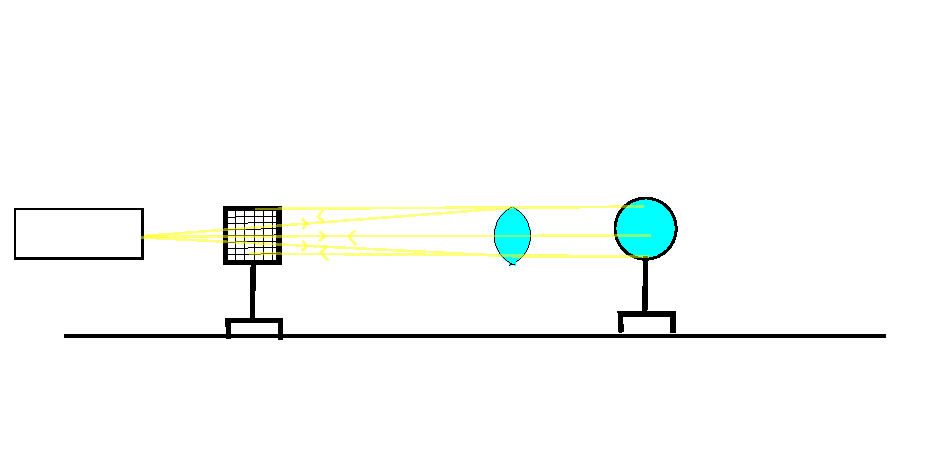
\includegraphics[width=0.9\linewidth]{autocollimation-refined.pdf}
\caption{Dispositif d'autocollimation pour la vérification des distances focales}
\label{fig:autocollimation}
\end{figure}

Nous avons obtenu les résultats suivants~:

\begin{table}[h]
\centering
\begin{tabular}{lrrr}
\toprule
 & \multicolumn{3}{c}{Lentille} \\
\cmidrule{2-4}
 & 1 & 2 & 3 \\
\midrule
Distance focale nominale (mm) & 100 & 150 & 200 \\
Distance focale mesurée (mm) & 104 & 155 & 208 \\
\bottomrule
\end{tabular}
\caption{Distances focales nominales et mesurées}
\label{tab:focal-distances}
\end{table}

\subsection{Construction d'un œil fictif}

Nous construisons un œil fictif avec une lentille convergente, qui représente le cristallin, et un écran blanc, qui représente la rétine~:

\begin{figure}[H]
\centering
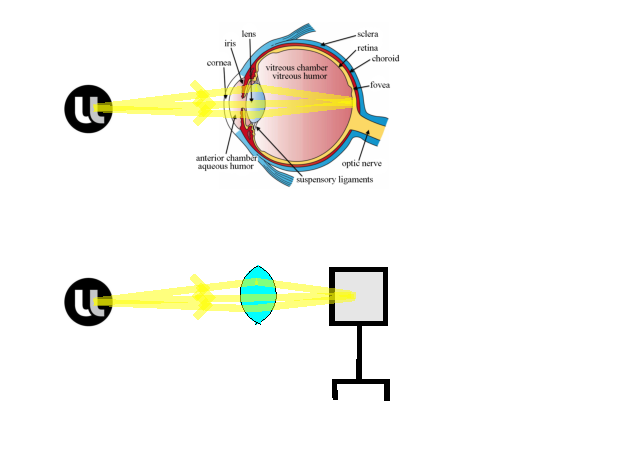
\includegraphics[width=0.9\linewidth]{eye-model.pdf}
\caption{Modèle de l'œil fictif}
\label{fig:eye-model}
\end{figure}

\subsubsection{Focalisation sur un objet à l'infini}

Nous construisons un scénario simulant la focalisation sur un objet considéré infiniment lointain (rayons lumineux arrivant parallèlement)~:

\begin{figure}[H]
\centering
\includegraphics[width=0.9\linewidth]{eye-vision-infinity.pdf}
\caption{Œil fictif focalisé à l'infini}
\label{fig:eye-infinite-focus}
\end{figure}

\subsubsection{Focalisation sur un objet proche (200 mm)}

Nous construisons un scénario simulant la focalisation sur un objet à 200~mm de l'œil~:

\begin{figure}[H]
\centering
\includegraphics[width=0.9\linewidth]{eye-vision-closeup.pdf}
\caption{Œil fictif focalisé sur un objet à 200~mm}
\label{fig:eye-closeup-focus}
\end{figure}

Avec la loi de Descartes
($\frac{1}{\overrightarrow{AO}} + \frac{1}{\overrightarrow{OA'}} = \frac{1}{\overrightarrow{OF'}}$),
nous avons calculé la nouvelle distance focale nécessaire pour obtenir une image nette sur la \og{}rétine\fg{} à 104~mm, ce qui est vérifié expérimentalement car une image nette est obtenue lorsque nous remplaçons la lentille convergente de distance focale nominale 200~mm (\og{}cristallin\fg{}) par une lentille convergente de distance focale nominale 100~mm.

\subsection{Expérimentation avec des loupes pour comprendre le mécanisme du grossissement optique}

Après avoir construit l'œil fictif et compris ses mécanismes optiques, nous tentons maintenant, à l'aide de lentilles convergentes (servant de loupes), de comprendre les mécanismes du grossissement optique.

Le dispositif expérimental est le suivant~:

\begin{figure}[H]
\centering
\includegraphics[width=0.9\linewidth]{magnifying-glass.pdf}
\caption{Dispositif expérimental avec loupe}
\label{fig:magnifying-glass}
\end{figure}

Ainsi, $O_{\text{œil}}A = 600~\text{mm}$ (choix arbitraire), œil focalisé à l'infini (simulé avec une lentille convergente de $f_{\text{nominal}} = 200~\text{mm}$).

À l'aide d'une règle, nous avons mesuré la taille de 11 carreaux verticaux du verre quadrillé à 24~mm, ce qui correspond à une moyenne de 2,182~mm par carreau.
Pour plus de commodité, nous isolons les quatre carreaux au-dessus du centre focal, ayant une hauteur théorique de 8,727~mm comme objet ($AB = 8{,}727~\text{mm}$)~:

\begin{figure}[H]
\centering
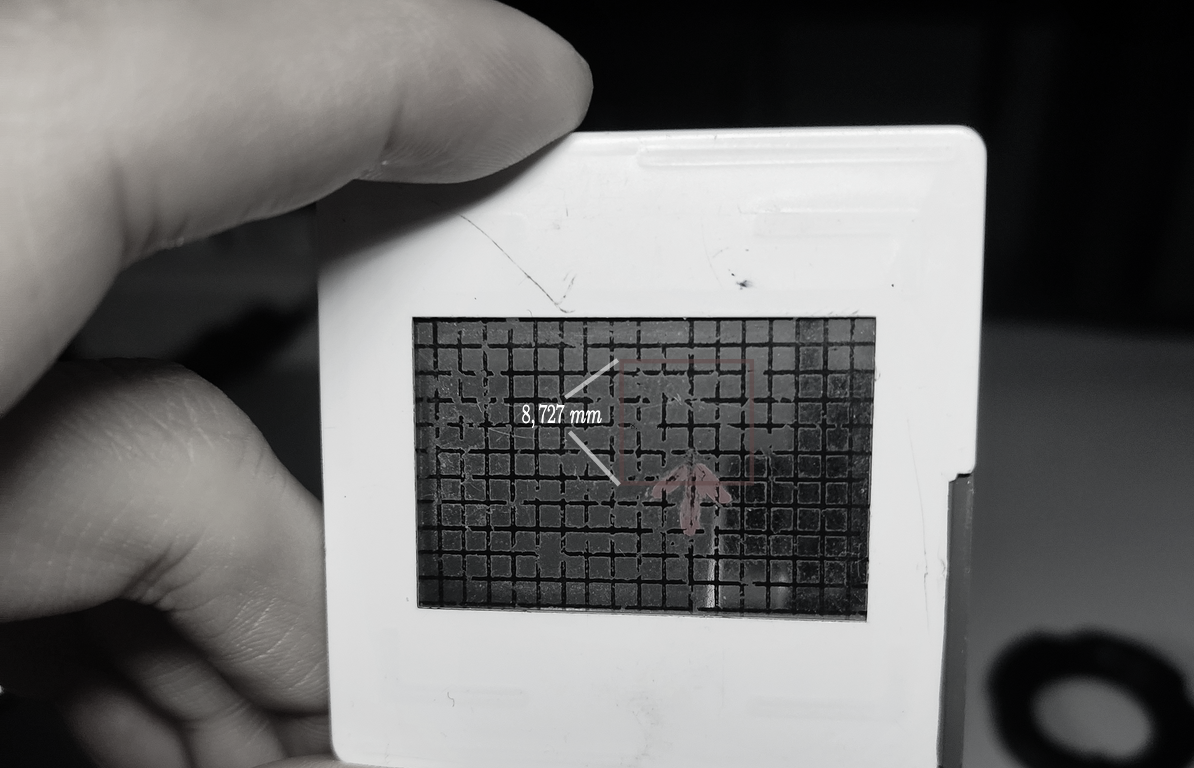
\includegraphics[width=0.9\linewidth]{grid-glass.png}
\caption{Verre quadrillé utilisé comme objet, avec quatre carreaux isolés au-dessus du centre focal}
\label{fig:grid-glass}
\end{figure}

Cela correspond à un angle d'observation $\alpha$ d'environ 0,0145 radians~:

\begin{figure}[H]
\centering
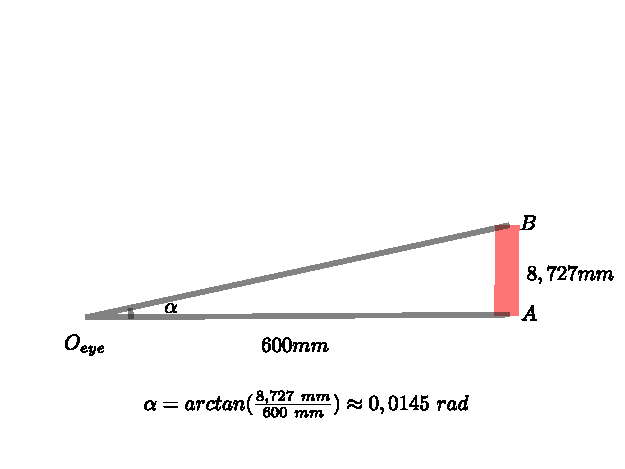
\includegraphics[width=0.9\linewidth]{observation-angle-object.pdf}
\caption{Angle d'observation $\alpha$ de l'objet}
\label{fig:observation-angle-object}
\end{figure}

Pour observer l'effet de grossissement, nous plaçons des lentilles convergentes de différentes longueurs focales entre le \og{}cristallin\fg{} et l'objet $AB$, en les déplaçant jusqu'à obtenir une image nette. Nous notons cette position $O$. $AB$ désigne l'objet (4 carreaux verticaux) et $A'B'$ désigne l'image projetée sur la \og{}rétine\fg{}.

Puisque l'œil est focalisé à l'infini, les rayons lumineux arrivant au \og{}cristallin\fg{} doivent être parallèles pour former une image nette sur la \og{}rétine\fg{}. Donc $\alpha' = \arctan\!\left(\frac{AB}{AO}\right)$. Ainsi la magnitude de grossissement $M = \frac{\alpha'}{\alpha} = \frac{\arctan\!\left(\frac{AB}{AO}\right)}{0{,}0145~\text{rad}}$~:

\begin{figure}[H]
\centering
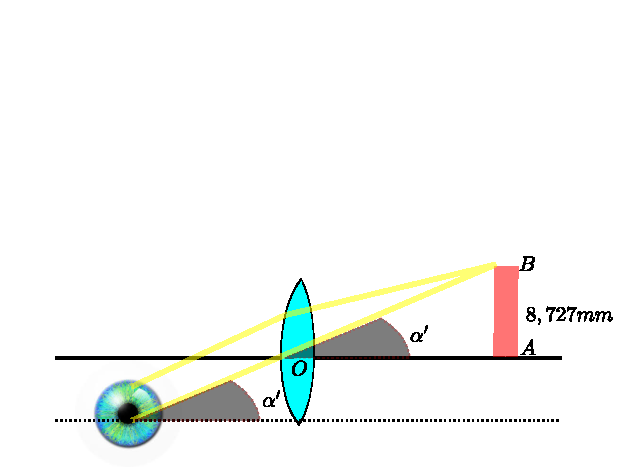
\includegraphics[width=0.9\linewidth]{magnification-magnitude.pdf}
\caption{Schéma de la magnitude de grossissement $M$}
\label{fig:magnification-magnitude}
\end{figure}

Expérimentalement, nous avons obtenu les mesures suivantes~:

\begin{table}[h]
\centering
\renewcommand{\arraystretch}{1.4}
\begin{tabular}{lrrrr}
\toprule
Mesure & \multicolumn{4}{c}{Loupe} \\
\cmidrule{2-5}
 & 1 & 2 & 3 & 4 \\
\midrule
Distance focale nominale $f$ (mm) & 100 & 150 & 300 & 500 \\
$OA$ (mm) & 142 & 186 & 260 & 392 \\
$A'B'$ (mm) & 9.0 & 7.7 & 6.0 & 5.0 \\
$\frac{A'B'}{AB}$ (calculé) & 1.031 & 0.882 & 0.688 & 0.573 \\
$M$ (calculé) & 4.22 & 3.22 & 2.31 & 1.53 \\
$\frac{M}{\frac{A'B'}{AB}}$ & 4.092 & 3.654 & 3.356 & 2.671 \\
\bottomrule
\end{tabular}
\caption{Mesures expérimentales du grossissement}
\label{tab:magnification}
\end{table}

À partir de ces résultats, nous pouvons attester que le cristallin humain \og{}rétrécit\fg{} les images avant de les transmettre à la rétine. Ayant remarqué que le champ de vision (représenté par le nombre de carreaux visibles sur l'écran) est de plus en plus limité avec des magnitudes de grossissement élevées, nous en déduisons que c'est délibéré afin de préserver le champ de vision lorsque nous regardons des objets bien plus grands que notre œil~!

De plus, en traçant $M$ en fonction de $\frac{1}{f}$~:

\begin{figure}[H]
\centering
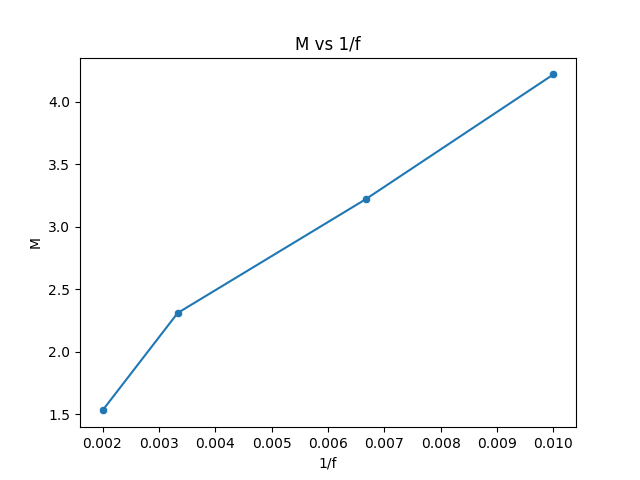
\includegraphics[width=0.9\linewidth]{M-f.png}
\caption{Graphe du grossissement $M$ en fonction de $\frac{1}{f}$}
\label{fig:M-f}
\end{figure}

Nous observons une relation quasi linéaire entre les deux, comme prévu.

\section{Conclusion}

Dans cette expérience, nous avons reconstruit un œil humain avec des analogues optiques géométriques pour comprendre comment un œil humain est capable de se focaliser sur des objets à différentes distances. Nous avons ensuite placé des lentilles convergentes de différentes distances focales devant notre œil analogique physique pour comprendre le fonctionnement des loupes. Nos résultats expérimentaux concordent avec les dérivations théoriques.

\section{Bibliographie}

\begin{thebibliography}{99}
\end{thebibliography}

\section{Annexe}

Code Python utilisé pour tracer $M$ en fonction de $\frac{1}{f}$~:

\begin{verbatim}
import seaborn as sns
import matplotlib.pyplot as plt
import pandas as pd

# Your data (converted to proper floats)
data = pd.DataFrame({
    "inv_f": [0.01, 0.00666666666666667, 0.00333333333333333, 0.002],
    "M": [4.22, 3.22, 2.31, 1.53]
})

# Plot
sns.scatterplot(data=data, x="inv_f", y="M")

# Optional: add line
sns.lineplot(data=data, x="inv_f", y="M")

plt.xlabel("1/f")
plt.ylabel("M")
plt.title("M vs 1/f")
plt.show()
\end{verbatim}

\end{document}
